%!TEX root = main.tex
\section{Introduction}

\subsection{Harmful Algal Blooms}
%%%%%%%%%%%%%%%%%%%%%%%%%%%%%%%%%%%%%%%%%%%
\begin{frame}{Harmful Algal Blooms}

\begin{columns}
	\column{0.5\textwidth}

	\begin{itemize}
		\item Increase in primary productivity
		\item Explosive growth of microscopic algae and cyanobacteria
		\item Toxin-producing genera
		\item Decrease biodiversity
		\item Anoxic environment
	\end{itemize}

	\column{0.5\textwidth}
	\begin{figure}
		\hspace*{-1cm}
		%\vspace*{-1cm}
		\includegraphics[width=2in,height=2in]{algal.jpg} \textsubscript{a}
		
	\end{figure}
\end{columns}
\footcitetext{[a]http://www.pme.com/wp-content/uploads/algal.jpg}
\end{frame}
%%%%%%%%%%%%%%%%%%%%%%%%%%%%%%%%%%%%%%%
\begin{frame}{HAB}

	\begin{itemize}
		\item Naturally occurring
		\item Exacerbate from anthropogenic causes \textsubscript{a}
		\item Worldwide issue
		\item Coastal environments
		\item Freshwater lakes
	\end{itemize}

\end{frame}
%%%%%%%%%%%%%%

\begin{frame}{Exposure Route}
	\begin{columns}
		\column{0.4\textwidth}
	\begin{itemize}
		\item Direct contact
		\item Aerosols
		\item Ingestion
		\begin{itemize}
			\item Seafood/Fish 
			\item Drinking water
			\item Algal supplements
		\end{itemize}
	\end{itemize}
	\column{0.5\textwidth}
	\begin{figure}
		\centering
		\includegraphics[width=2in]{swim.jpg}
	\end{figure}
\end{columns}
\footcitetext{[a], rastogi_cyanotoxin-microcystins:_2014}
\end{frame}
%%%%%%%%%%%%%%
\begin{frame}{Law and Regulation}
	\begin{columns}
		\column{0.4\textwidth}
	\begin{itemize}
		\item Safe Drinking Water Act \textsuperscript{a}  	
		\item Maximum Contaminant Level 
			\begin{itemize}
				\item Regulated and enforced
			\end{itemize}
		\item Contaminant Candidate List \textsuperscript{b} 
			\begin{itemize}
				\item ``More like guidelines''
			\end{itemize}
	\end{itemize}

	\column{0.5\textwidth}
	\begin{figure}
		\centering
		\includegraphics[scale=0.3]{warning.PNG}
	\end{figure}
	
	\end{columns}
	\footcitetext{[a], noauthor_guidelines_1998}
	\footcitetext{[b], usepa_drinking_2016}
\end{frame}
%%%%%%%%%%%%%%


\begin{frame}{Lake Erie 2014}
	\begin{figure}
		\centering
		\includegraphics[scale=0.35]{erie.jpg}
	\end{figure}
\hrule
{\tiny cdn.coastalscience.noaa.gov}
\end{frame}
%%%%%%%%%%%%%%
\begin{frame}{Possible causes}
	\begin{itemize}
		 
		\item Excess nutrient inputs
			\begin{itemize}
				\item Urbanization 
				\item Agriculture 
			\end{itemize}
		\item Invasive Zebra mussels (\emph{Dreissena polymorpha})
		\item Warmer climate
	\end{itemize}

	
\end{frame}
%%%%%%%%%%%%%%
\subsection{Cyanotoxins}
\begin{frame}{Cyanotoxins}

	\begin{itemize}
		\item Toxins
			\begin{itemize} 
				\item Microcystin and nodularin %\textsuperscript{1}
  				\item Cylindrospermopsin 
				\item Anatoxin 
				\item Saxitoxin 
				\item Produced nonribosomal polyketide synthase
			\end{itemize}
		\item Irritants
			\begin{itemize}
				\item Lipolysacharides \textsuperscript{a}
			\end{itemize}

	\end{itemize}
	\footcitetext{[a], moore_richard_cyanobacterial_1993}
\end{frame}
%%%%%%%%%%%%%%

\begin{frame}{Microcystin}

\begin{columns}
	\begin{column}{0.5\textwidth}

	\begin{itemize}
		\item Cyclic peptide
		\item 1000 Da
		\item Hepatoxin and carcinogenic
		\item Inhibits protein phosphatase
		\item Diverse structures 
		\item Intra-peritoneal LD\textsubscript{50} ranging from 25-150 $\mu$g/kg  \textsuperscript{a}
			\begin{itemize}
				\item Health Advisory (HA) of 4 $\mu$g/L over one day \textsuperscript{b}
			\end{itemize}
		\item Nonribosomally polyketide synthase (NRPS)
	\end{itemize}
	\end{column}
	\begin{column}{0.3\textwidth}
\begin{figure}[ht]
	\centering
	\hspace*{-1cm}
	\includegraphics[width=2in, height=2.2in]{../figures/Microcystin-LR.png}
\end{figure}
	\end{column}
\end{columns}
\footcitetext{[a], dittmann_cyanobacterial_2012}
\footcitetext{[b], usepa_draft_2016}
\end{frame}
%%%%%%%%%%%%%%
\begin{frame}{Cylindrospermopsin}

\begin{columns}
	\column{0.5\textwidth}
	\begin{itemize}
		\item Polycyclic uracil derivative\textsuperscript{a} 
		\item Toxicity not fully understood\textsuperscript{b}
			\begin{itemize}
				\item Covalently binds to DNA/RNA 
				\item Inhibits protein synthesis %\textsuperscript{3} 
			\end{itemize}
		\item LD\textsubscript{50} of 150-200 $\mu$/kg over 5 days\textsuperscript{c}
			\begin{itemize}
				\item Health Advisory of 8 $\mu$g/L over one day\textsuperscript{d}
			\end{itemize}
	\end{itemize}
	\column{0.5\textwidth}
	\begin{figure}
		%\hspace*{-10cm}
		\centering
		\includegraphics[width=2in]{cylindro.png}
	\end{figure}
\end{columns}
\footcitetext{[a], moreira_cylindrospermopsin:_2013}
\footcitetext{[b], kittler_1._2014}
\footcitetext{[c], shaw_cylindrospermopsin_2000}
\footcitetext{[d], usepa_draft_2016}
\end{frame}
%%%%%%%%%%%%%%
\begin{frame}{Anatoxin-a}
\begin{columns}
	\column{0.5\textwidth}
	\begin{itemize}
		\item Alkaloid 
		\item Known as Very Fast Death Factor \textsuperscript{a}
			\begin{itemize}
				\item Binds to acetylcholine receptor
				\item Paralysis 
				\item Respiratory failure
			\end{itemize}
		\item LD\textsubscript{50} of 300-375 $\mu$g/kg over 24 \textsuperscript{b}
	\end{itemize}
	\column{0.5\textwidth}
	\begin{figure}
		%\hspace*{-10cm}
		\centering
		\includegraphics[width=2in]{anatoxin.png}
	\end{figure}
	\hspace*{-3cm}
\end{columns}
\footcitetext{[a], codd_cyanobacterial_1999}
\footcitetext{[b], shaw_cylindrospermopsin_2000}
\end{frame}
%%%%%%%%%%%%%%
\begin{frame}{Saxitoxin}
\begin{columns}
	\column{0.5\textwidth}
	\begin{itemize}
		\item Neurotoxin  
		\item Sodium channel blocker
		\item Paralytic shellfish poisoning
			\begin{itemize}
				\item Respiratory failure 
				\item Mouth-to-mouth resuscitation 
			\end{itemize}
		\item LD\textsubscript{50} of 2-10$\mu$g/kg over 24 h 
	\end{itemize}
	\column{0.5\textwidth}
	\begin{figure}
		%\hspace*{-10cm}
		\centering
		\includegraphics[width=2in]{saxitoxin.png}
	\end{figure}
\end{columns}
\footcitetext{saoudi_management_2017}
\end{frame}
%%%%%%%%%%%%%%
\subsection{Survey Objectives}
\begin{frame}{Objectives}
	\begin{itemize}
		\item Investigate drivers of Harmful Algal Blooms 
		\item Evaluate different techniques of detection 
		\item Do lake's with heavy urbanized watershed prone to have more cyanotoxins? 
		\item Do lake's with Zebra mussels are more at risk of cyanotoxins?
	\end{itemize}
\end{frame}
%%%%%%%%%%%%%%
\section{Survey Methods}
\subsection{Sampling}
\begin{frame}{Surveyed Lakes}

\begin{figure}
	\centering
	\includegraphics[width=0.8\textwidth,height=\textheight]{../figures/Overview.png}
	\caption{Sampled Lakes}
\end{figure}

\end{frame}

%%%%%%%%%%%%%%%%%%%%%%%%%%
\begin{frame}{Water Sampling}

	\begin{itemize}
		\item Sampled each lake once a month
		\item Collected water samples
			\begin{itemize}
				\item Waded in towards the center of the lake until water reaches waist height
				\item Water samples are taken roughly 10-20cm below the surface
			\end{itemize}
		\item Quickly transported back
		\item Analyzed ASAP
	\end{itemize}

\end{frame}
%%%%%%%%%%%%%%%%%%%%%%%%%%%%%
\begin{frame}
	\frametitle{Sampler}
\begin{columns}
	\column{0.5\textwidth}
	\begin{itemize}
		\item 3 PVC plates for collecting Zebra Mussels 
		\item Slotted PVC tube to hold SPATT 
		\item Installed on riparian owner's dock or on labeled floats  
		\item From July 2017 to October 2017
		\item Temperature/Light loggers 
		\item Mature Zebra mussels are collected in October
	\end{itemize}
	\column{0.5\textwidth}
	\begin{figure}
		\includegraphics[width=2.3in,angle=-90]{sampler.jpg}
	\end{figure}
\end{columns}


\end{frame}



%%%%%%%%%%%%%%%%%%%%%%%%%%%%%%
\begin{frame}{SPATT}

\begin{columns}
	\column{0.5\textwidth}
	\begin{itemize}
		\item Solid phase adsorbtion toxin tracking 
		\item Dianon HP-20 
		\begin{itemize}
			\item Styrene-divinylbenzene copolymer beads
		\end{itemize} 
		
		\item Sachet filled with resin
		\item Cyanotoxin adsorb onto the resin
		\item Left for one month
	\end{itemize}

	\column{0.5\textwidth}
	\begin{figure}
		\includegraphics[width=2.3in,angle=-90]{bag.jpg}
	\end{figure}

\end{columns}

\end{frame}

%%%%%%%%%%%%%%%%%%%%%%%%%%%%%

\subsection{Chemical Analysis}

%%%%%%%%%%%%%%%%%%%%%%%%%%%%%%%
\begin{frame}{Nutrients}
	\begin{itemize}
\item Colormetric analysis
\begin{itemize}
		\item P 
			\begin{itemize}
				\item Total and dissolved orthophosphorus (\ch{PO4-})
			\end{itemize}
		\item Nitrate+nitrite-N 
			\begin{itemize}
				\item Azo dye
			\end{itemize}
		\item Ammonia-N 
			\begin{itemize}
				\item Indophenol blue
			\end{itemize}
		\item Total Kejdlahl nitrogen 
			\begin{itemize}
				\item Azo dye
			\end{itemize}
		\item Total Phosphorus
			\begin{itemize}
				\item Antimony-phospho-molybdate complex
			\end{itemize}
	\end{itemize}
\end{itemize}
	

\end{frame}

%%%%%%%%%%%%%%%%%%%%%%%%%%%%%%
\begin{frame}{LC-MS/MS}
	\begin{itemize}
		\item Grab Samples: 
		\begin{itemize}
			\item Freeze/thaw 3x for cell lysis 
			\item Filtered samples with 96 well block 
		\end{itemize}
		\item SPATT: 
		\begin{itemize}
			\item Once retrieved, cyanotoxins are soaked in 85\% methanol with 10mM ammonium formate
		\end{itemize}
		\item Analyzed 12 different microcystin congeners	
	\end{itemize}
	\begin{figure}
		\includegraphics[width=\textwidth]{../figures/LCMS_CONGENERS.png}
	\end{figure}
\end{frame}

%%%%%%%%%%%%%%%%%%%%%%%%%%%%%
\begin{frame}{ELISA}
	\begin{itemize}
		\item Enzyme-Linked Immunosorbant Assay
		\item Abraxxis\textsuperscript{a}
	\end{itemize}

	
\end{frame}
\footcitetext{[a], noauthor_saxitoxin_nodate}
\subsection{Statistical Analysis}
%%%%%%%%%%%%%%%%%%%%%%%%%%%%%
\begin{frame}{Geospatial Analysis}

\end{frame}
%%%%%%%%%%%%%%%%%%%%%%%%%%%%%
\section{Results}
\subsection{Toxin Results}
\begin{frame}{Cyanotoxins}
	\begin{itemize}
		\item No detection of Cylindrospermopsin or Saxitoxin (gene)
		\item Anatoxin in Brighton Lake (2.80$\mu$g/L) in August 2017
		\item Few instances of microcystin above health advisory from grab samples
			\begin{itemize}
				\item Belleville, Brighton, Cadillac, Ford, Hudson and Wixom Lake
				
			\end{itemize}

			
	\end{itemize}
\end{frame}
%%%%%%%%%%%%%%%%%%%%%%%%%%%%%
\begin{frame}
	\frametitle{Microcystin-ELISA and LC-MS/MS}


	\begin{figure}
		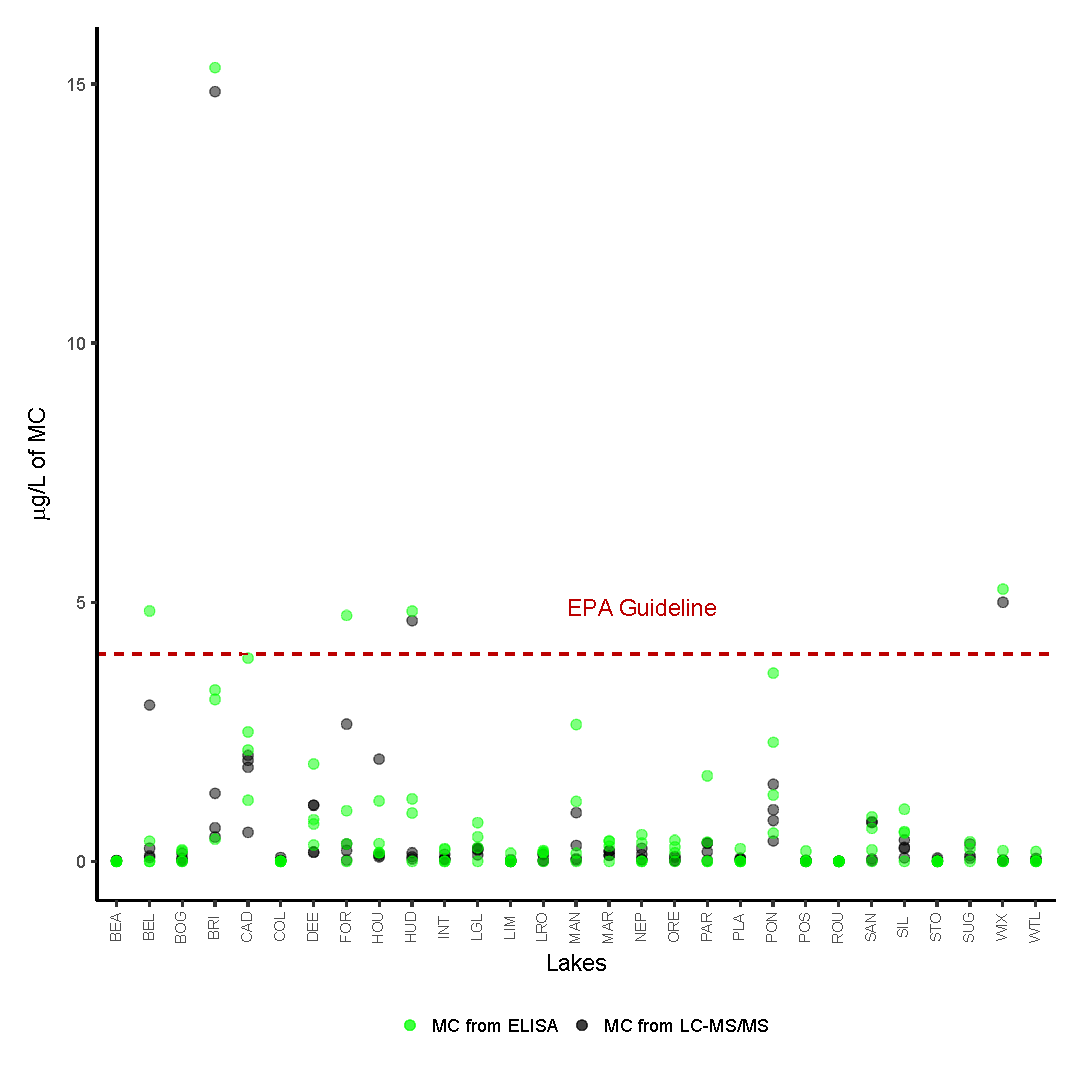
\includegraphics[width=\textwidth,height=0.9\textheight]{../figures/Microcystin.eps}
	\end{figure}

\end{frame}
%%%%%%%%%%%%%%%%%%%%%%%%%%%%%%%%%%%%%%%
\begin{frame}
	\frametitle{Microcystin-LC-MS/MS}


	\begin{figure}
		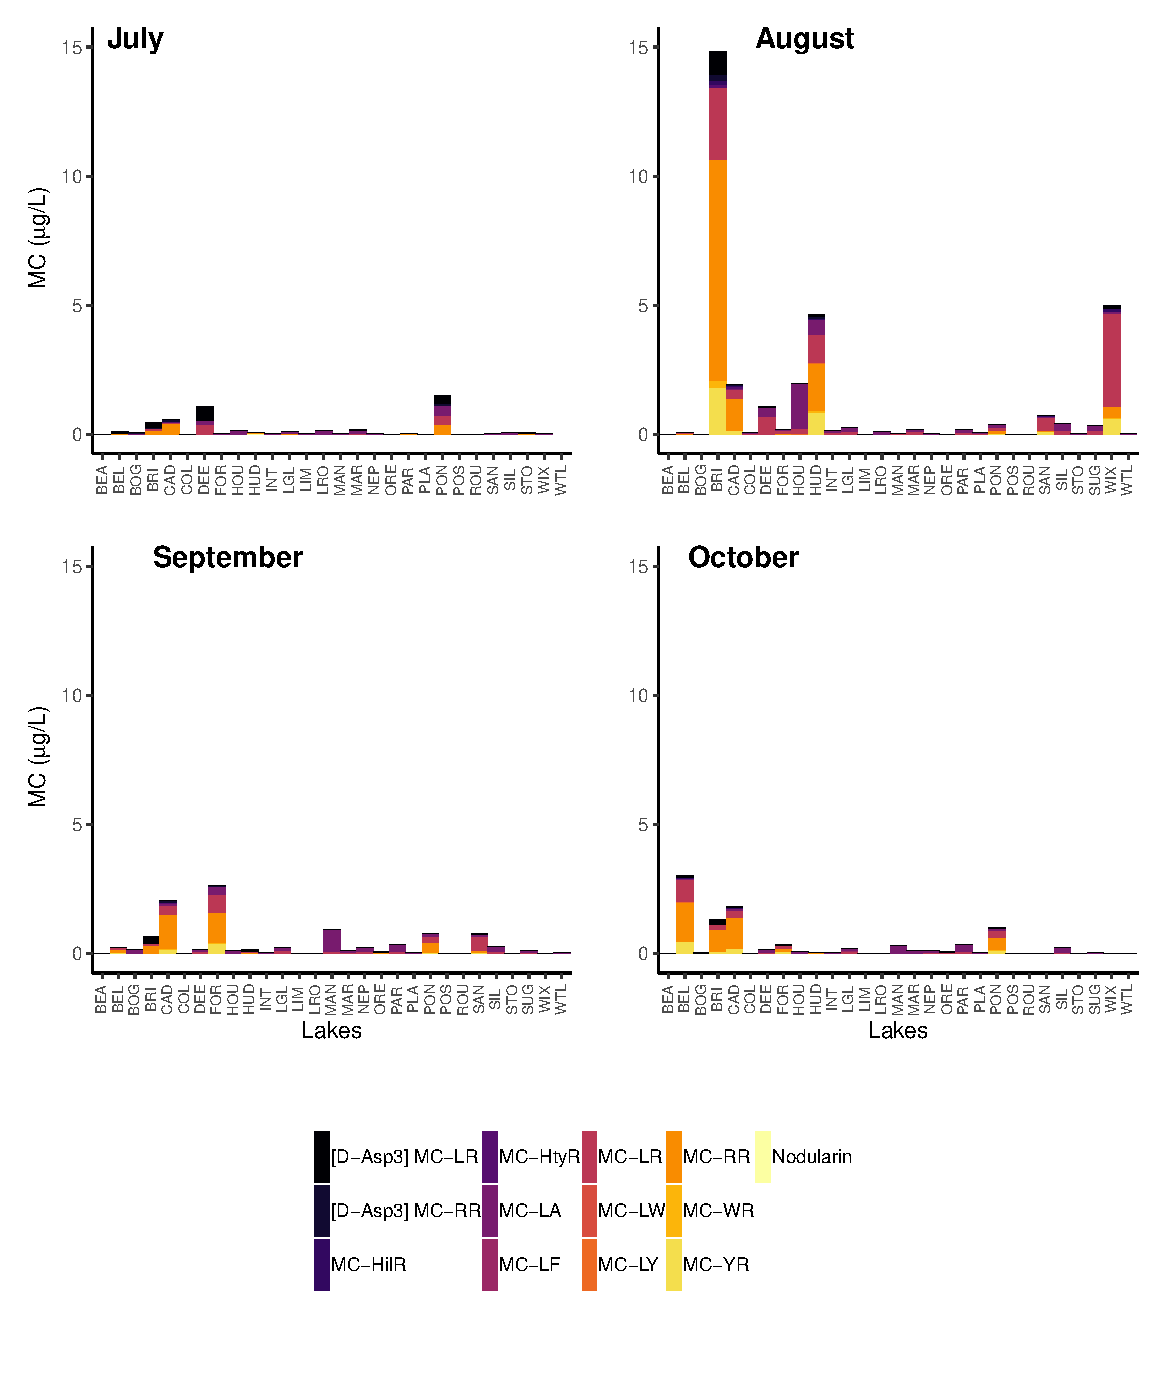
\includegraphics[width=\textwidth,height=0.99\textheight]{1month.eps}
	\end{figure}

\end{frame}

%%%%%%%%%%%%%%%%%%%%%%%%%%%%%%%%%%%%%

%%%%%%%%%%%%%%%%%%%%%%%%%%%%%%%%%%%%%
\begin{frame}
	\frametitle{Microcystin-SPATT}

	\begin{figure}
		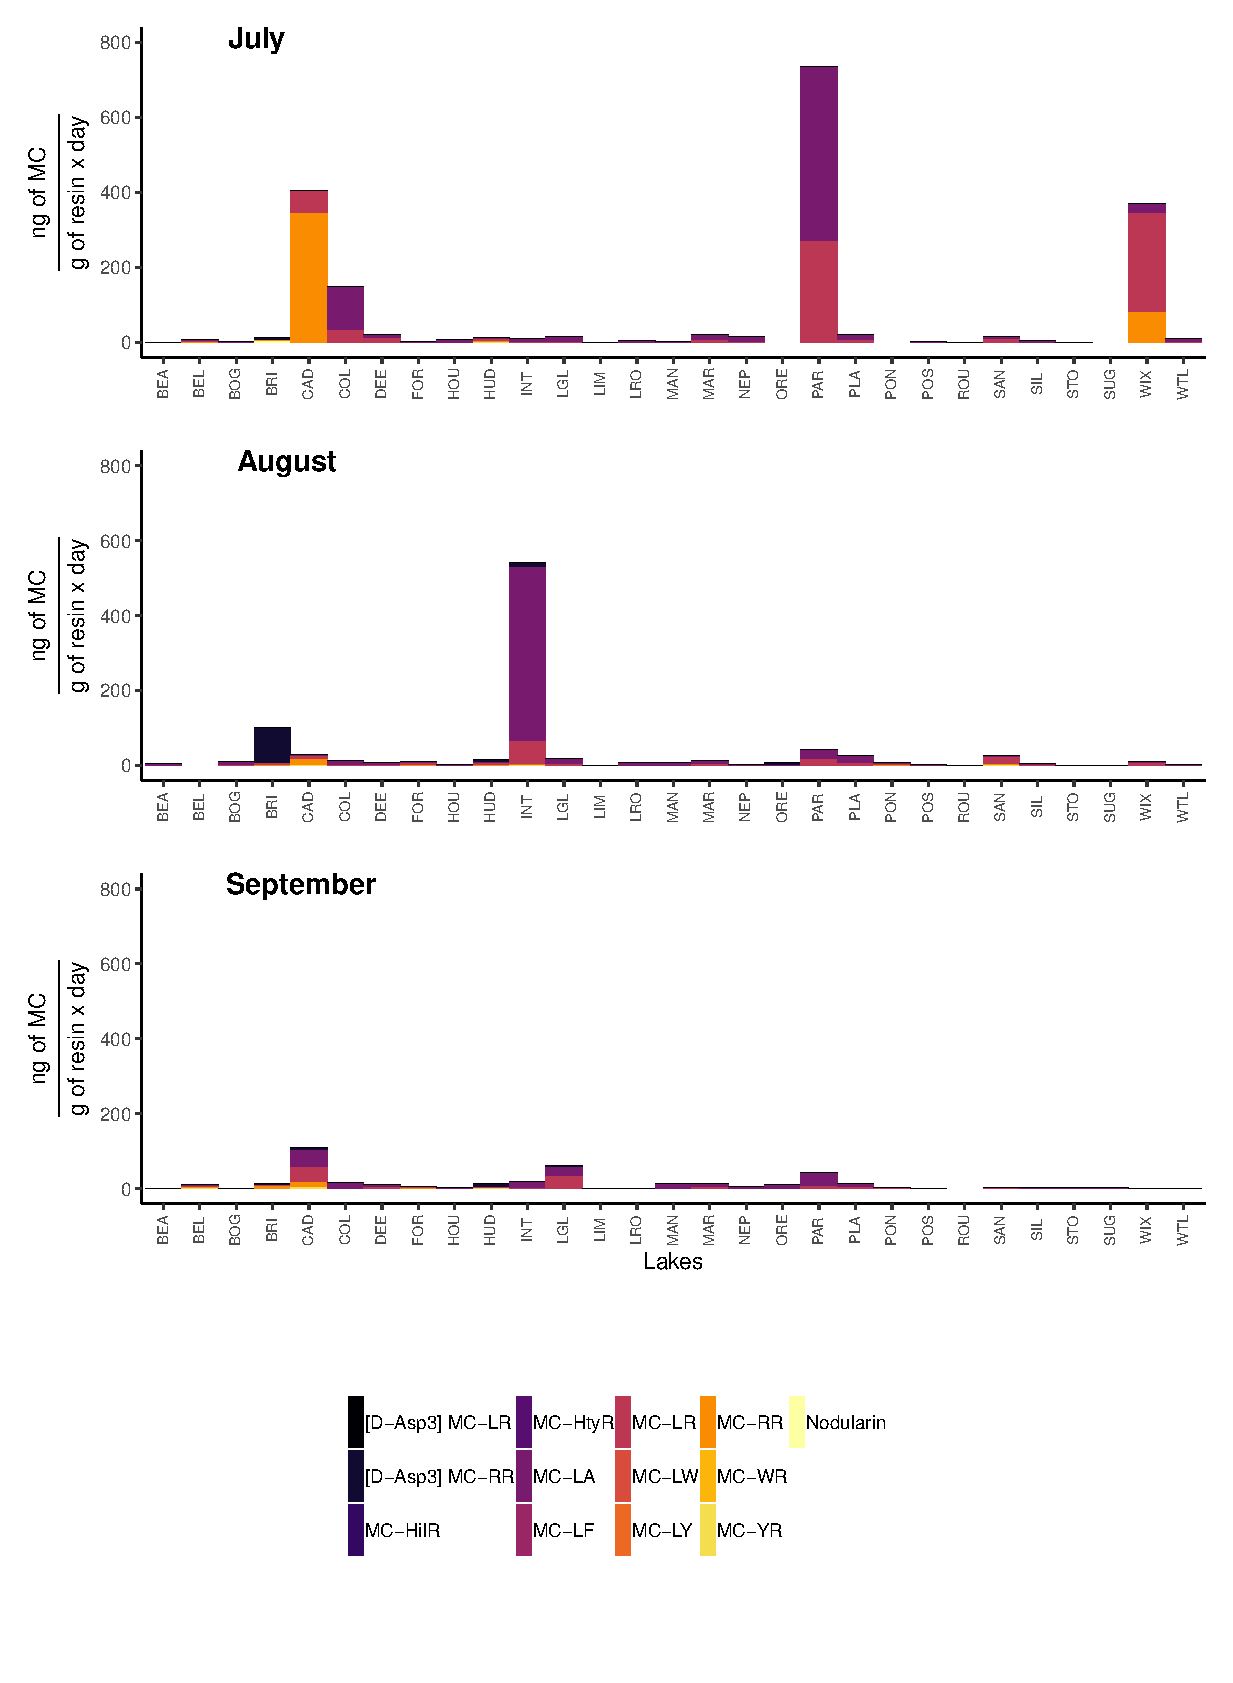
\includegraphics[width=\textwidth,height=1.04\textheight]{1spatter.eps}
	\end{figure}
\end{frame}

%%%%%%%%%%%%%%%%%%%%%%%%%%%%%%%%%%%%%%%
\begin{frame}
	\frametitle{Comparison}
	\begin{figure}
		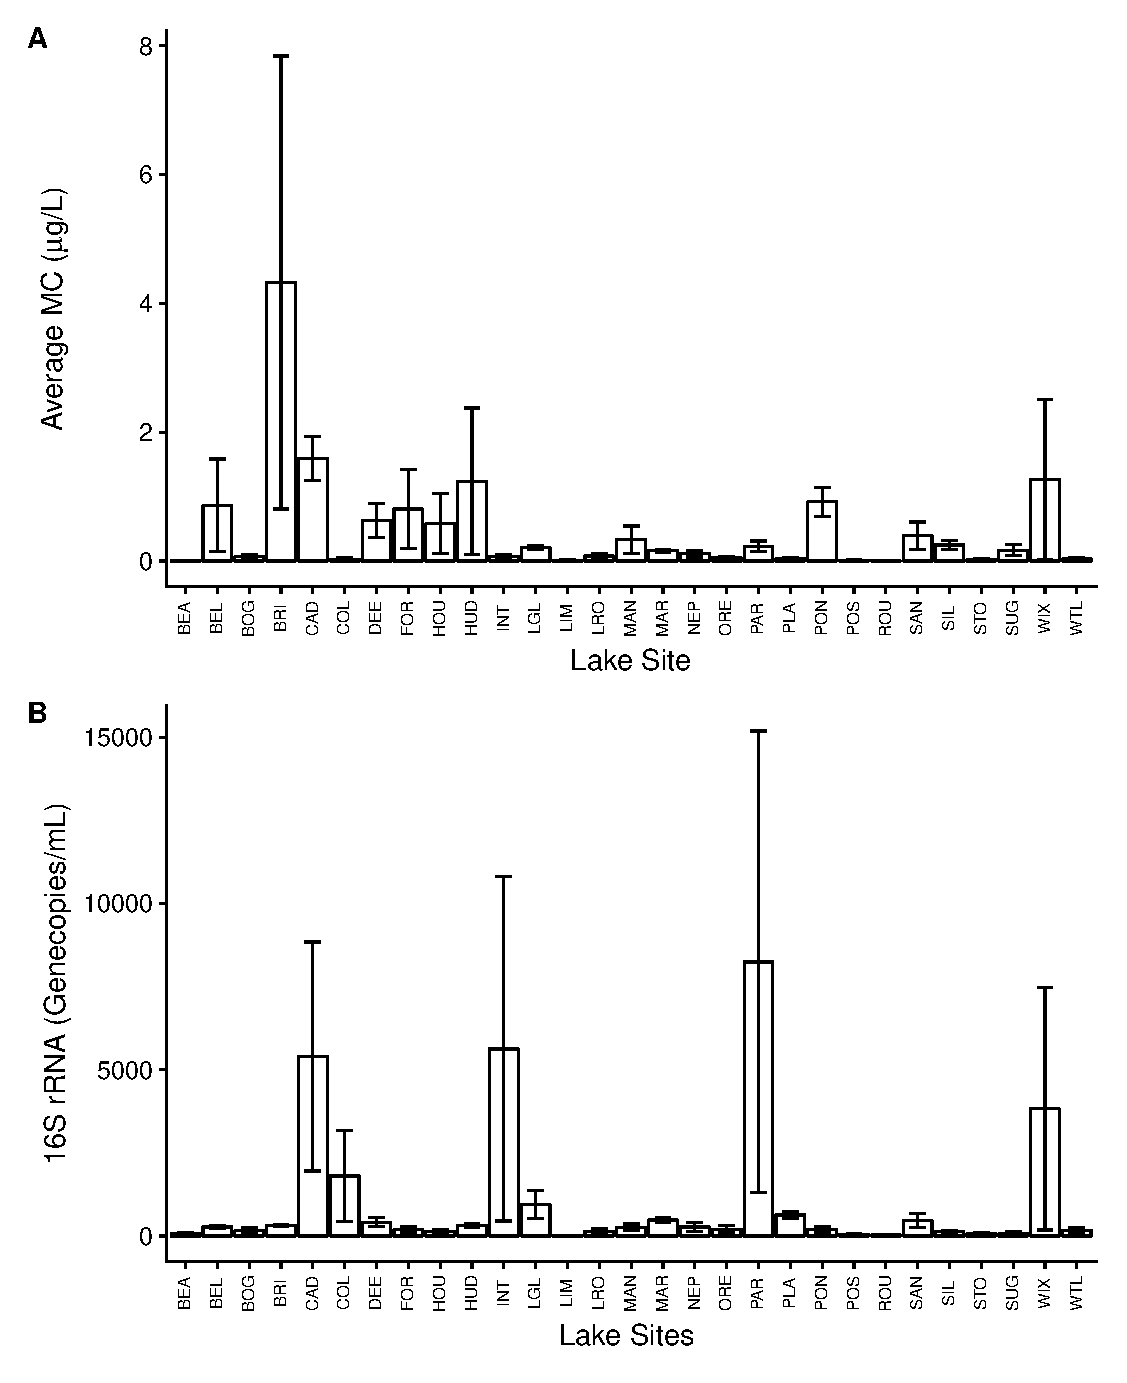
\includegraphics[width=\textwidth, height=\textheight]{../figures/responsecombine.eps}
	\end{figure}
\end{frame}

<++>
%%%%%%%%%%%%%%%%%%%%%%%%%%%%%%%%%%%%%%%%
\subsection{Environmental Drivers}
\begin{frame}
	\frametitle{Land-Use}
		
\end{frame}



%%%%%%%%%%%%%%%%%%%%%%%%%%%
\section{Conclusion}
\begin{frame}{Conclusion}
	\begin{itemize}
		\item Most of the sampled lakes were low, with a few exceptions 
		\item Did not find any clear environmental drivers 
		\item ELISA and LC-MS/MS agree very well 
		\item Did not find association between urbanization and algal blooms 
		\item Measuring turbidity may provide a preliminary screening tool
	\end{itemize}

	
\end{frame}
%%%%%%%%%%%%%%%%%%%%%%%%%%%%%%%%%%
\begin{frame}
	\frametitle{Lesson learned}

	\begin{itemize}
		\item Survey is too broad 
			\begin{itemize}
				\item Focus on fewer lakes
			\end{itemize}
		\item Take more samples at each lake 
			\begin{itemize}
				\item Samples at different depths 
				\item Frequent sampling 
				\item 
			\end{itemize}
		\item "All models are false"
	\end{itemize}

	

\end{frame}


%%%%%%%%%%%%%%%%%%%%%%%%%%%%%
\begin{frame}{Acknowledgment}

	\begin{itemize} 
		\item My lab team mates: Brian Spies, Andrew Herrpich, Brayden Metcalf, Mikaela Cantu and Alyssa
		\item Jason Sckrabulis, Ryan Mcwhinnie, Melissa Ostrowski, Patrick Long, James Willis
		\item Dr.David Szlag and Dr. Thomas Raffel
		\item Westrick Group at Wayne State University
		\item Ben Southwell at Lake Superiour State University
		\item Michigan Department Environmental Quality
		\item Oakland University and the Chemistry Department
	\end{itemize}
\end{frame}
\begin{frame}
\begin{center}
Thank You
\end{center}
\end{frame}
\section{Appendix}
\begin{frame}
	\frametitle{Appendix1}
	\begin{figure}
	\includegraphics[width=\textwidth]{Isotherm.png}
	\end{figure}	

\end{frame}
%%%%%%%%%%%%%%%%%%%%%%%%%%%%%%%%%%%%%%
\begin{frame}
	\frametitle{Water Chemistry}
	\begin{figure}
		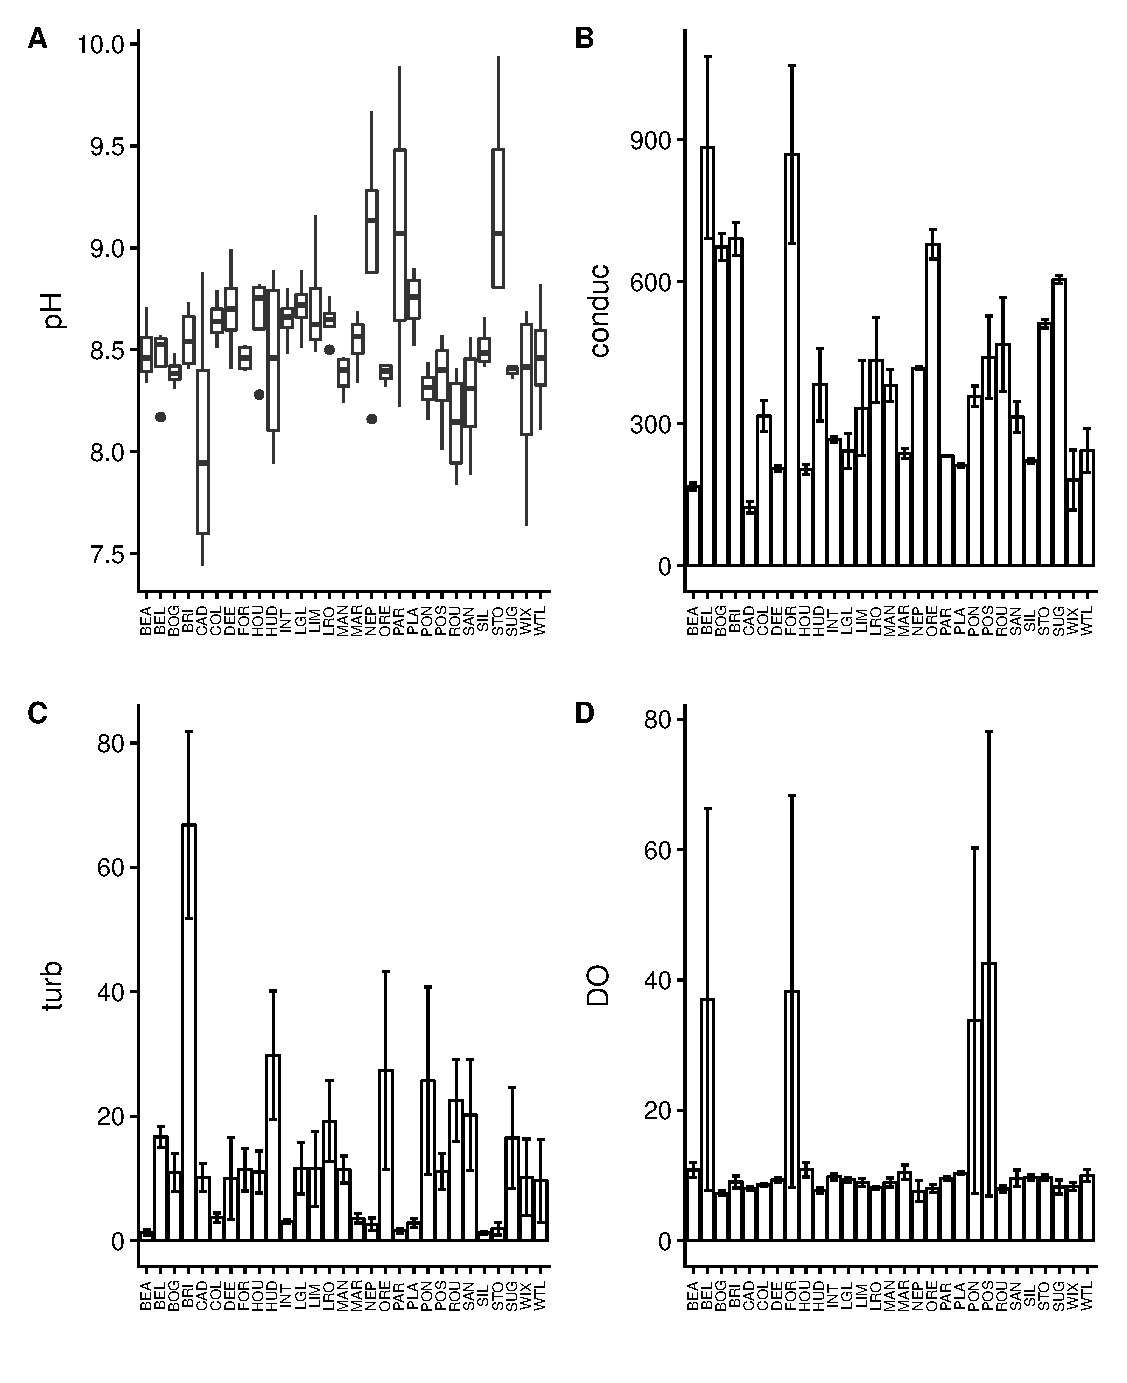
\includegraphics[width=0.7\textwidth,height=\textheight]{../figures/watboxplotlake.eps}
	\end{figure}
\end{frame}
%%%%%%%%%%%%%%%%%%%%%%%%%%%%%%%%%%%%%%%%	
\begin{frame}
	\frametitle{Nutrients}

	\begin{figure}	
		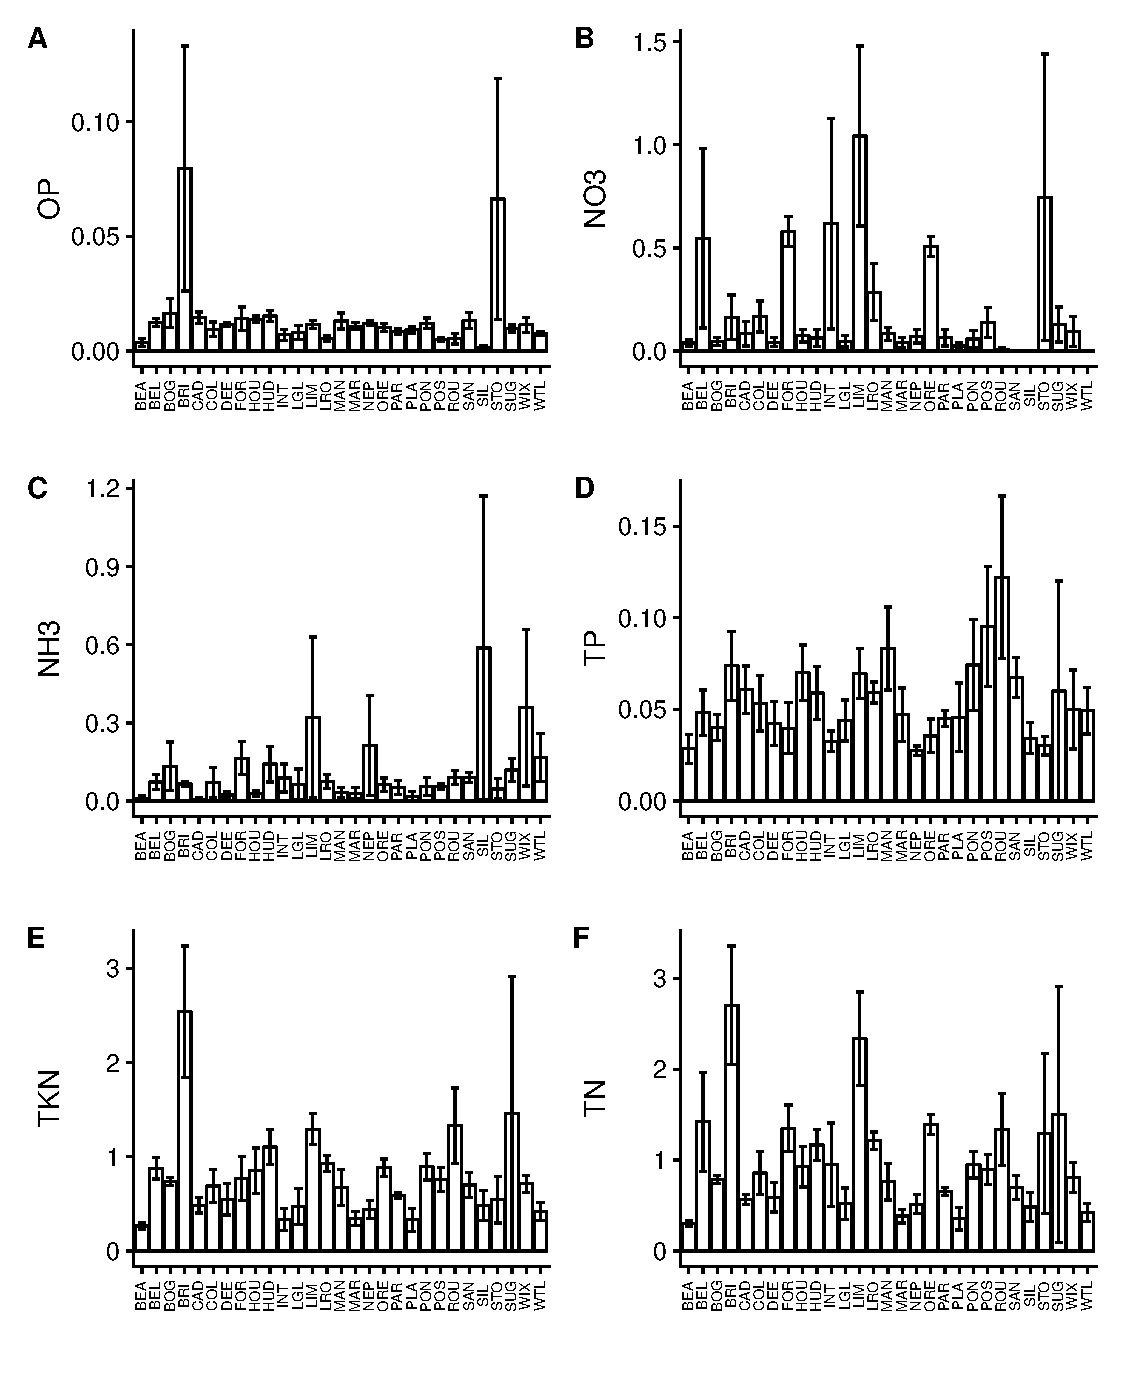
\includegraphics[width=0.7\textwidth, height=\textheight]{../figures/nutboxplotlake.eps}
	\end{figure}

\end{frame}



\begin{frame}
	\frametitle{Congener Stats-Grab}

\resizebox{4in}{!}{

\begin{table}
   \tiny
   \begin{tabular}{@{\extracolsep{2pt}}lccccccc}
   \\[-1.8ex]\hline
   \hline \\[-1.8ex]
   Statistic & \multicolumn{1}{c}{N} &           
    \multicolumn{1}{c}{Mean} & \multicolumn{
   1}{c}{St. Dev.} & \multicolumn{1}{c}{Min} &   
    \multicolumn{1}{c}{Pctl(25)} & \
   \multicolumn{1}{c}{Pctl(75)} &                 
    \multicolumn{1}{c}{Max} \\
  \hline \\[-1.8ex]
  Nodularin & 114 & 0.0003 & 0.002 & 0.000 & 0. 
    000 & 0.000 & 0.021 \\
  {[D-Asp3]}MC-RR & 114 & 0.006 & 0.028 & 0.000 
    & 0.000 & 0.000 & 0.255 \\
  MC-RR & 114 & 0.185 & 0.855 & 0.000 & 0.000 & 
    0.018 & 8.552 \\
  MC-YR & 114 & 0.046 & 0.202 & 0.000 & 0.000 & 
    0.000 & 1.799 \\
  MC-HtyR & 114 & 0.002 & 0.012 & 0.000 & 0.000 
    & 0.000 & 0.107 \\
  MC-LR & 114 & 0.142 & 0.447 & 0.000 & 0.000 & 
    0.087 & 3.570 \\
  {[D-Asp3]}MC-LR & 114 & 0.027 & 0.107 & 0.000 
    & 0.000 & 0.000 & 0.902 \\
 MC-HilR & 114 & 0.004 & 0.019 & 0.000 & 0.000 
    & 0.000 & 0.150 \\
  MC-WR & 114 & 0.005 & 0.029 & 0.000 & 0.000 & 
    0.000 & 0.302 \\
 MC-LA & 114 & 0.088 & 0.196 & 0.000 & 0.005 & 
    0.105 & 1.729 \\
  MC-LY & 114 & 0.0004 & 0.002 & 0.000 & 0.000  
    & 0.000 & 0.024 \\
 MC-LW & 114 & 0.000 & 0.000 & 0.000 & 0.000 & 
    0.000 & 0.000 \\
  MC-LF & 114 & 0.0002 & 0.001 & 0.000 & 0.000  
    & 0.000 & 0.012 \\
  MC Sum from LC MS/MS  & 114 & 0.505 & 1.580 & 
    0.000 & 0.018 & 0.266 & 14.857
   \\
  MC from ELISA & 115 & 0.747 & 1.784 & 0 & 0 & 
    0.6 & 15 \\
  \hline \\[-1.8ex]
  \multicolumn{8}{r}{Values are expressed       
    as($\mu$g of MC*${L^{-1}}$)} \\
  \end{tabular}

  \end{table}
}
\end{frame}



%%%%%%%%%%%%%%%%%%%%%%%%%%%%%%%%%%%%%%%%%%%%%%%%%%%%%%%%%%

\begin{frame}
	\frametitle{SPATT-Table}
	\resizebox{4in}{!}{

\begin{table}  	
\tiny 
\begin{tabular}{@{\extracolsep{5pt}}lccccccc} 
\\[-1.8ex]\hline 
\hline \\[-1.8ex] 
Statistic & \multicolumn{1}{c}{N} & \multicolumn{1}{c}{Mean} & \multicolumn{1}{c}{St. Dev.} & \multicolumn{1}{c}{Min} & \multicolumn{1}{c}{Pctl(25)} & \multicolumn{1}{c}{Pctl(75)} & \multicolumn{1}{c}{Max} \\ 
\hline \\[-1.8ex] 
{[D-Asp3]}MC-RR & 91 & 0 & 0 & 0 & 0 & 0 & 0 \\ 
MC-RR & 91 & 5 & 37 & 0 & 0 & 0 & 346 \\ 
Nodularin & 91 & 0 & 1 & 0 & 0 & 0 & 5 \\ 
MC-YR & 91 & 0 & 1 & 0 & 0 & 0 & 5 \\ 
MC-HtyR & 91 & 0 & 0 & 0 & 0 & 0 & 1 \\ 
MC-LR & 91 & 12 & 40 & 0 & 0 & 6 & 272 \\ 
{[D-Asp3]}MC-LR & 91 & 2 & 10 & 0 & 0 & 0 & 92 \\ 
MC-HilR & 91 & 0 & 0 & 0 & 0 & 0 & 2 \\ 
MC-WR & 91 & 0 & 0 & 0 & 0 & 0 & 0 \\ 
MC-LA & 91 & 18 & 69 & 0 & 1 & 9 & 466 \\ 
MC-LY & 91 & 0 & 0 & 0 & 0 & 0 & 3 \\ 
MC-LW & 91 & 0 & 0 & 0 & 0 & 0 & 0 \\ 
MC-LF & 91 & 0 & 0 & 0 & 0 & 0 & 1 \\ 
MC Sum from LC MS/MS & 91 & 36 & 109 & 0 & 3 & 16 & 737 \\ 
MC from ELISA & 60 & 112 & 257 & 0 & 11 & 69 & 1,050 \\ 
\hline \\[-1.8ex] 
\multicolumn{8}{r}{Values are expressed as (ng of MC / gram of resin)} \\ 
\end{tabular} 
\end{table} 	
}

\end{frame}
